
\chapter{图形与衬底}

\section{素数之别于合数}

想想简单的印符操作能把握概念,不免有点令人奇怪。迄今为止我们已把握到的概念是加法,这说来还不显得有多怪。可我们现在的目标是做出一个形式系统,使定理都是$"P"x$的形状,其中字母$x$代表一个短杠符号串,并且只有当短杠符号串中的短杠数目是素数时才能成为定理。这样,$"P"---$是个定理,而$"P"----$则不是。怎么能用印符操作来做这件事?首先,说清楚所谓印符操作是什么意思是很重要的。我们能用的东西都已在"WJU"系统和"pq"系统中给出了,所以我们实际上只需列出我们所允许的种种操作:
\begin{enumerate}
\item 读入并认出有限的符号集合中任何一个符号;
\item 写下属于该集合的任何一个符号;
\item 把任何一些那样的符号从一处复制到另一处;
\item 删除任何一些那样的符号;
\item 检测一个符号是否与另一个符号相同;
\item 保存并使用一列以前产生的定理。
\end{enumerate}
这张表有点多余,不过没关系。重要的是它很明显只涉及一些极简单的能力,它们远比区分素数与非素数的能力简单得多。那么,我们怎样才能组合这些操作,构造一个形式系统,在其中素数能与合数区别开呢?

\section{"tq"系统}

第一步该是试图去解决一个简单些、但却与此有关的问题。我们可以做一个与"pq"系统类似的系统,差别是这次我们表示的是乘法。我们称之为"tq"系统,“"t"”代表“乘”(英文是times)。进一步还得说明,我们用$X$、$Y$、$Z$分别表示短杠符号串$x$、$y$、$z$中的短杠数目(注意我在此特别用心地区分符号串与它所包含的短杠数目)。现在我们希望符号串$x"q"y"t"z$是个定理,当且仅当$X$等于$Y$乘以$Z$。例如,$------"q"--"t"---$应该是个定理,因为$2$乘以$3$等于$6$,但$---"q"-"t"--$不应是个定理。"tq"系统可以像"pq"系统一样很容易地刻划——就是说,只用一个公理模式和一条推理规则:
\begin{thm}{公理模式}
$x"q"x"t"-$是一个公理,对任何一个短杠符号串$x$都是如此。
\end{thm}

\begin{thm}{推理规则}
设$x$、$y$、$z$都是短杠符号串。设$x"q"y"t"z$是个已有的定理。那么,$xy"q"y"t"z-$是个新的定理。
\end{thm}
下面是定理$------"q"--"t"---$的推导:
\begin{enumerate}
\setaitem{.4\linewidth}
\aitem $--"q"--"t"-$       \>(公理)
\aitem $----"q"--"t"--$    \>(用推理规则,(1)作为已有定理)
\aitem $------"q"--"t"---$ \>(用推理规则,(2)作为已有定理)
\end{enumerate}
若注意每次使用推理规则时最后的那个短杠符号串是怎样增长的,你就可以预言,如果想导出一个最后有十个短杠的定理,就得接连用九次推理规则。

\section{把握合数}

乘法是个比加法稍难对付的概念,现在已由印符操作“把握住”了,就像艾舍尔的《释放》里的那些鸟。素数性质怎么样呢?这里有个看来聪明的计划:使用"tq"系统,定义一集形如$"C"x$的新定理来刻划合数:
\begin{thm}{规则}
设$x$、$y$、$z$是短杠符号串。如果$x"q"y-"t"z-$是定理,则$"C"x$是定理。
\end{thm}

这能行得通,因为:说$X$($x$中的短杠数目)是合数,仅当它是两个大于$1$的数的乘积——即,是$Y+1$($y-$中的短杠数目)和$Z+1$($z-$中的短杠数目)的乘积。我可以提出某种“惟方式”的论证来为这条规则辩护,因为你是人,想知道为什么会有这样一条规则。假如你是完全以“机方式”运转的,你就不会需要任何论证了,因为"J"方式工作者只是机械地、快乐地遵循规则,从不产生疑问。

由于你以"W"方式工作,你会趋于把符号串与对符号串的解释相混淆。你知道,一旦你从你所操作的符号里找到“意义”,事情就会变得相当混乱。你不得不和你的自我作斗争,阻止自己把符号串“$---$”认作数目$3$。对形式化的要求,在第一章里或许显得令人迷惑不解(因为它看上去如此显然),在这里却变得相当复杂,并且很关键。这里的实质在于防止你自己把"W"方式与"J"方式相混淆,或者换一种说法,在于防止你自己把算术事实与印符定理相混淆。

\section{对素数的非法刻划}

一个很诱人的做法是从"C"型定理直接跳到"P"型定理,就是草拟下面这样一个规则:

草拟的规则:设$x$是一个短杠符号串。如果$"C"x$不是个定理,那么$"P"x$是个定理。

这里致命的缺陷是:$"C"x$是否是个定理并非一个显明地表达出的印符操作。要确定"WU"不是"WJU"系统的定理,你必须到系统的外面去……对这个草拟的规则也是如此。这是一个完全违反了形式系统观念的规则,它要求你非形式化地进行操作——就是说,在系统之外进行操作。印符操作\pnum{6}允许你查看以前所发现的定理的储备,可是这条草拟的规则却要求你去查看假定的一张“非定理表”。但要想产生这样一张表,你必须得在系统之外进行一番推理——这种推理是说明为什么某些符号串不能在系统内生成。当然很可能有那么一个另外的形式系统,能纯粹通过印符手段产生“非定理表”。事实上,我们的目标恰恰就是要找这么一个形式系统。但上面草拟的那个规则不是个印符规则,必须放弃。

这一点非常重要,因此我们还得再稍微多说几句。在我们的"C"系统里(包括"tq"系统及定义"C"型定理的那条规则),我们有形如$"C"x$的定理,其中“$x$”像通常一样代表一个短杠符号串。也有形如$"C"x$的非定理(这些就是当我说“非定理”时所指的东西,虽然$"tt"-"Cqq"$以及其它乱七八糟不规矩的东西也显然是非定理)。区别在于,定理含有合数数目的短杠,非定理含有素数数目的短杠。现在所有的定理都具有一个共同的“形式”,也就是说,都源自一个共同的印符规则集。那么,在同一意义上,所有的非定理是否也具有一个共同“形式”呢?下面是一列"C"型定理,不带推导。它们后面括号中的数字只是记录其中的短杠数目。
\begin{align*}
 & "C"---- \quad (4) \\
 & "C"------ \quad (6) \\
 & "C"-------- \quad (8) \\
 & "C"--------- \quad (9) \\
 & "C"---------- \quad (10) \\
 & "C"------------ \quad (12) \\
 & "C"-------------- \quad (14) \\
 & "C"--------------- \quad (15) \\
 & "C"---------------- \quad (16) \\
 & "C"------------------ \quad (18) \\
 & \qquad \vdots
\end{align*}

这张表中的“洞”是那些非定理。重复那个早先的问题:那些洞也具有某种共同的“形式”吗?对,也不对。无可否认的是它们都具有某种印符特性,但我们是否要称之为“形式”却是不清楚的。理由是那些洞仅仅是以否定的方式定义的——它们是被一列以肯定的方式定义的东西所排除的那些东西。

\section{图形和衬底}

这让人想起艺术中对“图形”和“衬底”的著名区分。当一个图形或“正空间”(例如,一个人形、一个字母、一个静物)画在画框里时,不可避免地也就画上了与它互补的形状——也称作“衬底”、“背景”或“负空间”。在多数绘画中,这种图形与衬底的关系不起多少作用。艺术家对衬底远不如对图形那么感兴趣。但有时候,艺术家也会对衬底同样感兴趣。

有一种漂亮的汉字书写方式就是着意摆弄这种图形与衬底的区分。下面的\fig{15}就是用这种笔画来传达信息的。猛一看,它像是一团团随便涂上的墨斑,但若你退后一些盯着它看一会,你会突然发现,有四个汉字出现在这里……

\begin{figure}
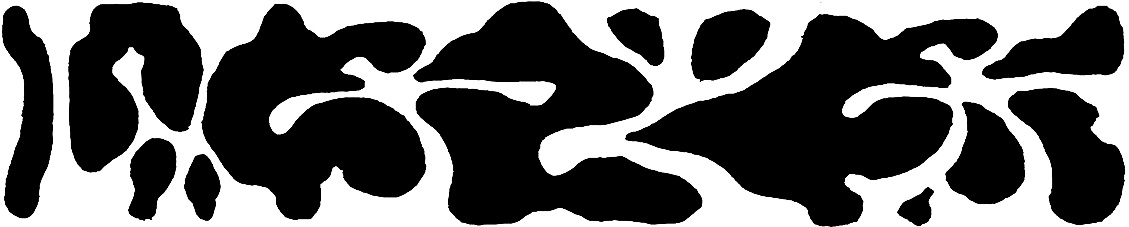
\includegraphics{img_015.png}
\caption[“以子之矛”。]
  {刘皓明绘。}
\end{figure}

类似的效果可以在我画的《以烟为号》(\fig{139})中看到。沿着这条思路下去,你可以考虑一下下面这个谜题:你能否想个什么办法作一幅画,使其中的图形及衬底都是图形?

\begin{figure}
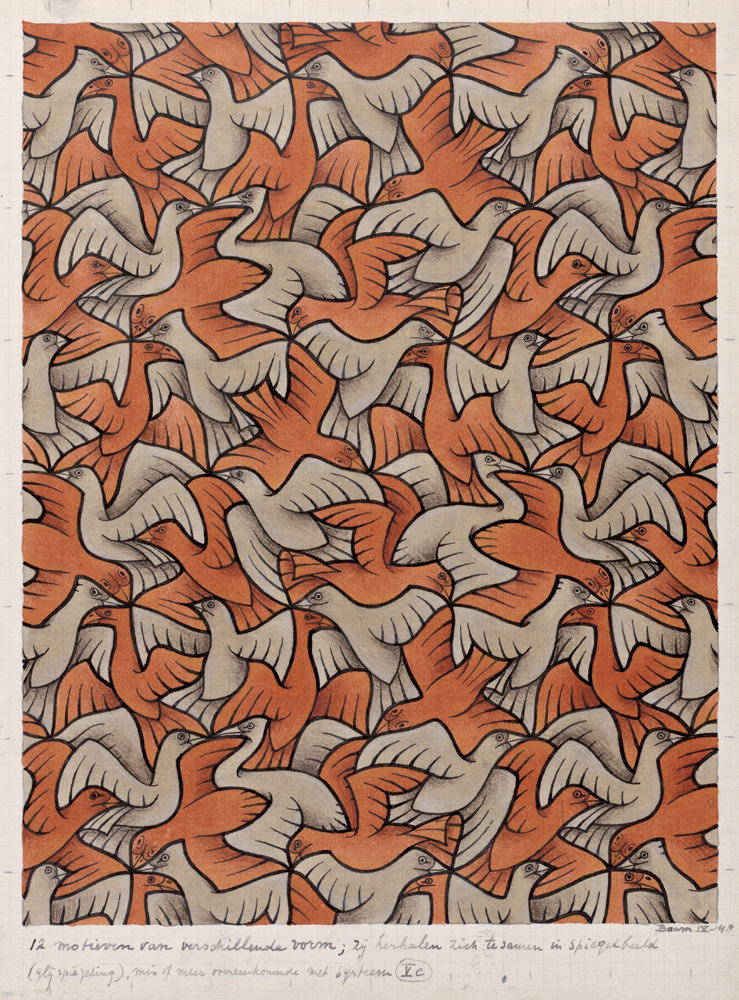
\includegraphics{img_016.jpg}
\caption[以鸟作瓦,艾舍尔作。]
  {以鸟作瓦,艾舍尔作(选自1942年的速写本)。}
\end{figure}

现在我们来正式地区分两类图形:流畅可画出的和倍流畅的(顺便说明,这些词是我自己的用语——并非通常都这么用)。在流畅可画出的图形中,衬底仅仅是绘画过程中顺带的副产品。而在倍流畅的图形中,衬底本身也可视为一个图形。这通常都需要艺术家的精心构思。“倍流畅”的“倍”字表示前景和背景都是流畅地画出来的——图形是“双倍流畅的”。在倍流畅图形中,图形与衬底的每道分界线都是双刃宝剑。艾舍尔是画倍流畅图形的大师——例如,他倍流畅地画出的那些漂亮的鸟(\fig{16})。

我们这种区分并非像数学里那么精确。谁能肯定地说一幅画中的衬底就一定不是个图形?一旦指出这一点,那么几乎任何衬底都有它自己的价值。在这种意义下,每个图形都是倍流畅的。但那不是我这用语的意图。我们对可识别的形状都有种自然直觉的观念。前景与背景是否都是可识别的形状?如果是,那么这幅画是倍流畅的。当你看大多数线条画的衬底时,你会发现它们是极难识别的。这就证明了:

\begin{block}
存在可识别的形状,其负空间是不可识别的形状。
\end{block}

用更为“技术性”的词语来说,就是:

\begin{block}
存在非倍流畅的流畅可画出图形。
\end{block}

\begin{figure}
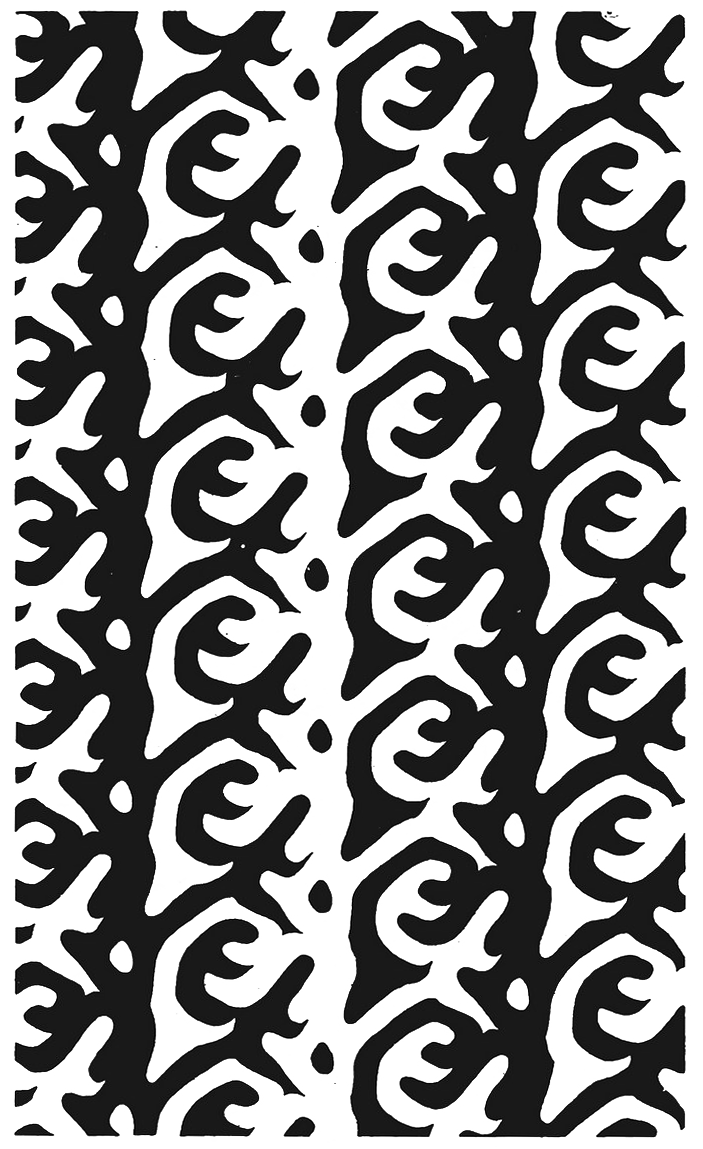
\includegraphics[height=.9\textheight]{img_017.png}
\caption[FIGURE-FIGURE图形,斯科特·凯姆作。]
  {FIGURE-FIGURE图形,斯科特·凯姆作\pnum{1975}。你能看出其中的单词吗?}
\end{figure}

对于前面说到的那个谜题,斯科特·凯姆给出了一个解:他直接在英语单词FIGURE(“图形”的意思)上作文章。\fig{17}就是他作的画,我称之为FIGURE-FIGURE图形。如果你看了这幅画中白的部分再看黑的部分,你看到的都会是FIGURE,就是说,你总是看到“图形”,而永远看不到“衬底”。这是个倍流畅图形的典范。在这幅巧妙的画中,可以有两种不等价的方式来刻划黑的部分:
\begin{enumerate}
\item 作为白的部分的负空间;
\item 作为白的部分的变形副本(通过将白的部分涂黑并平移而得到)。
\end{enumerate}
(在FIGURE-FIGURE图形这种特殊情况下,两种刻划确实是等价的——但在大多数黑白图画中,两者不会等价。)将来在第八章,当我们构思我们的印符数论(即TNT)时,我们将希望能用两种类似的方式来刻划所有的数论假陈述的集合:
\begin{enumerate}
\item 作为TNT的所有定理的集合的负空间;
\item 作为TNT的所有定理的集合的变形副本(通过否定每个TNT定理而得到)。
\end{enumerate}
但这个希望将破灭,因为:
\begin{enumerate}
\item 在非定理组成的集合中有真理。
\item 在所有被否定的定理组成的集合之外有“假理”。
\end{enumerate}
在第十四章里你会看到这是为什么,以及是怎样发生的。同时,也请你琢磨琢磨用图形表达出来的这种境况(\fig{18})。

\begin{figure}
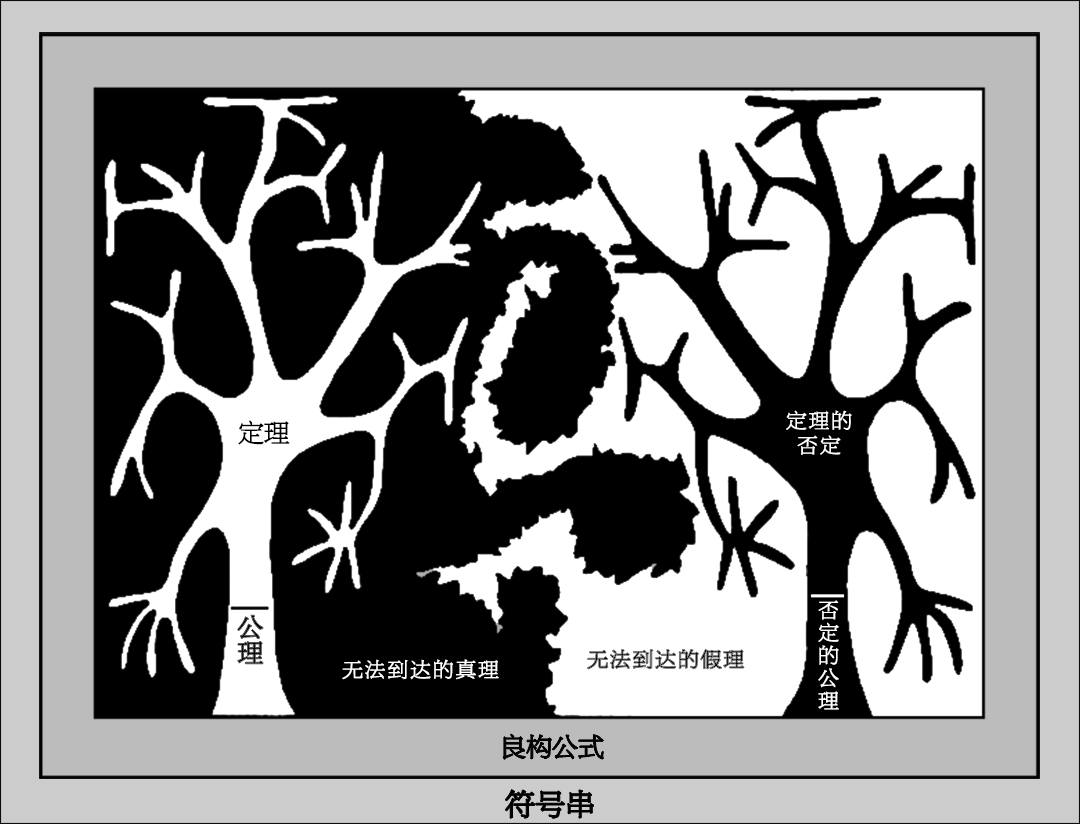
\includegraphics{img_018.png}
\caption[各类串之间的关系图示。]
  {这张图形象地描绘了TNT中各种符号串之间的关系。最大的方框代表所有TNT符号串的集。次一级的方框代表所有良构的TNT符号串的集,在它里面有TNT的所有语句的集。现在事情开始有趣了。所有定理的集合画成了一棵树,树干代表公理的集合。选树来作象征是因为它展现出来的递归生长的模式:新的枝条不断地从旧的里面生长出来。手指一样的枝条探到了约束区域(真理集)的各个角落,然而永远无法完全覆盖这个区域。真理和“假理”之间的分界线有意地提示出一种曲折随机的海岸线,无论你如何仔细地察看,总是有更细微的结构,因而不可能用有穷的方式精确地加以描述。(参见孟德尔布劳特所著《碎片》。)对应的树代表定理的否定的集:它们都是假的,但它们整个却无法充满假陈述的空间.[作者绘]}
\end{figure}

\section{音乐中的图形与衬底}

在音乐中也可以找到图形与衬底。类比之一就是旋律与伴奏之间的区别——因为在某种意义上讲,旋律总是处在我们注意力的前沿,而伴奏是第二位的。因此当我们在一部乐曲的较低声部发现可识别的旋律时会很惊奇。这种乐曲在巴罗克以后的音乐中不太常见。和声通常不被当作是前景。但在巴罗克音乐中——尤其是在巴赫的音乐里——各个声部,不论是高是低或在中间,都是起“图形”作用的。从这个意义上讲,巴赫的曲子可以称为“倍流畅的”。

音乐中还有另一种图形衬底的区分:强半拍与弱半拍之间的区分。如果你为一个小节里的音符打拍子:“一‡嗒,二‡嗒,三‡嗒,四‡嗒”,多数旋律音符会落在数字上,而不是“嗒”上。但有时候,一段旋律会刻意地落在各个“嗒”上,纯粹追求这种效果。例如,肖邦有几首钢琴练习曲就有这种旋律。巴赫的曲子里也有——特别是他的无伴奏小提琴奏鸣曲和帕蒂塔,以及无伴奏大提琴组曲。

在这些曲子里,巴赫用各种办法使两个或更多的曲调同时进行。有时他让独奏乐器用“双弦”奏法——两个音同时奏,有时他让一个声部落在强半拍上,而另一个声部落在弱半拍上,这样听起来就能把它们区分开来,听到两个不同的旋律盘旋交织,互相协调地融合在一起。不用说,巴赫还远不只停留在这种水平的复杂程度上……

\section{递归可枚举集之别于递归集}

现在让我们把图形与衬底的概念带回到形式系统这个领域。

在前面的例子里,正空间的角色是由C型定理来扮演,负空间的角色是由带素数个短杠的符号串来扮演的。到目前为止,我们找到的用印符规则表示素数的仅有手段是把它们视为负空间。那么,是否有什么手段——我不在乎多复杂——能把素数作为正空间表示出来——就是说,作为某种形式系统的定理的集合?

这里,不同人的直觉给出不同的回答。我还能生动地记起当初为了体会正的刻划与负的刻划之间的区别,我是怎样地着迷而大伤脑筋的。那时我相当肯定地认为不仅素数,而且任何能被负地表示出来的数的集合都同样能正地表示出来。我这个信念背后的直觉可以用一个问题来表达:“一个图形与其衬底怎么会不带有完全相同的信息?”在我看来,它们体现了同样的信息,只是以互补的两种方式对信息编码而已。在你看来正确的回答是什么?

结果就素数而言我是对的,但对一般情形来说我错了。这使我很吃惊,而且就是到了今天我也仍继续感到吃惊。那是这样一个事实:

\begin{block}
存在一个形式系统,其负空间(非定理集)不是任何一个形式系统的正空间(定理集)。
\end{block}
后来证明了,这个结果与哥德尔定理具有同样的深度——因此我的直觉出错是不奇怪的。我,正像二十世纪初的数学家们一样,期望着形式系统与自然数的世界比实际上更可预测。用更为技术性的术语来说,上面的结果就是:

\begin{block}
存在非递归的递归可枚举集。
\end{block}
“递归可枚举”这个词(通常缩写为“r.e.”)是我们那个艺术上的“流畅可画出”概念的数学对应物——而“递归”则是“倍流畅”的对应物。一集符号串是“r.e.”的,意思是它能按照印符规则来生成——例如,C型定理的集合、"WJU"系统的定理集合——其实,任何形式系统的定理集都是这样。这可以和“图形”概念,作为“能按照艺术规则生成的线条的集合”(且不管那是些什么样的规则),作个比较。而一个“递归集”就像是个其衬底也是个图形的图形——不仅它r.e.,它的补集也r.e.。

上述结果导致:

\begin{block}
存在一些形式系统,它们没有用印符规则表述的判定过程。
\end{block}
怎么会得出这样的结论呢?很简单。一个用印符规则表述的判定过程是一种分辨定理与非定理的测试方法。有了这样的测试,我们就能系统地生成所有的非定理。方法很简单:把所有的符号串排成一列,对它们逐个施用这个测试,除掉那些非良构串及那些定理。这就相当于一个生成非定理集合的印符方法了。但按照前面的那个论断(在这里我们当作信念而接受),对于某些系统这是不可能的。因此我们必须下结论:并非所有的形式系统都有用印符规则表述的判定过程。

假定我们找到了一个自然数的集合$T$(相应于“图形”),能用某种形式的方法生成——就像合数那样。假定它的补集是$C$(相应于“衬底”)——就像素数那样。$T$和$C$加在一起就是全部自然数了。我们知道一个产生$T$集中所有的数的规则,但我们知道没有同样的产生$C$集中所有的数的规则。了解下面这一点是很重要的:如果$T$集中的元素总能按长度递增的方式生成,那么我们总是能够刻划$C$。问题在于许多r.e.集的生成方式是以任意的次序添加元素的,因此你永远无法知道某个数被跳过之后过了很长时间会不会被收进来,如果你只要稍稍再等一会的话。

对于那个艺术问题:“所有的图形都是倍流畅的吗?”我们回答了“否”。现在我们看到了,对于数学中的类似问题:“所有的集合都是递归的吗?”我们必须同样地回答否。带着这样的观察,让我们回到那个费解的词“形式”。让我们再摆出我们的图形集T和衬底集$C$。我们可以承认集$T$中所有的数都有某种共同的“形式”——但对于集$C$中的数也能这么说吗?这是个奇怪的问题。当我们着手对付一个无限的集合——自然数——的时候,通过去掉某个子集而产生的洞大概是很难用什么显明的方式来定义的。因此它们或许不带有任何共同的特性或“形式”。分析到最后,用不用“形式”这个词成了口味问题——但思考这件事是很有意思的。也许最好是不去定义“形式”,而把它留给灵活的直觉。

这里有个供思考的谜题,它与上面谈的事情紧密相关:你能刻划出下面这样的整数集合(或者它的负空间)吗?
\[
1\quad 3\quad 7\quad 12\quad 18\quad 26\quad 35\quad 45\quad 56\quad 69
\ldots\ldots
\]
这个序列与FIGURE-FIGURE图形有何相似?

\section{素数作为图形而非衬底}

最后,让我们来看看生成素数的形式系统。它是怎么做到的?技巧是跳过乘法,直接把不可整除性当作要正面表示的东西。下面是一个公理模式和一条规则,它们产生的定理可以准确地表达一个数不整除("BZC")另一个数这个概念:

\begin{thm}{公理模式}
$xy"BZC"x$,其中$x$和$y$是短杠符号串。
\end{thm}
例如,$-----"BZC"--$,这里“$--$”代替了$x$,而“$---$”代替了$y$。

\begin{thm}{规则}
若$x"BZC"y$是个定理,则$x"BZC"xy$是个定理。
\end{thm}

如果你把这个规则用两次,你就能生成下面这个定理:
\[
-----"BZC"------------
\]
这可以解释成“$5$不整除$12$”。但$--"BZC"------------$不是个定理。要是你试图生成它,会出什么问题?

现在为了确定一个给定的数是素数,我们得建立某种关于它的不可整除性的知识。特别地,我们希望知道它不能被这样一些数整除:$2$、$3$、$4$、等等,如此下去,直到比那个数本身小$1$的数。但我们在形式系统里不能含糊不清地说“等等”之类的话。我们必须明白地说淸楚。我们大概会要有一种方式以这个形式系统的语言来说出“数$Z$在直到$X$的数内没有因子(记作$z"MY"x$)”,意思是在$2$和$X$之间没有能整除$Z$的数。这是能做到的,但要点技巧。如果你愿意,你可以自己想一想。

下面是解决方案:

\begin{thm}{规则}
如果$--"BZC"z$是个定理,则$z"MY"--$是个定理。
\end{thm}
\begin{thm}{规则}
如果$z"MY"x$与$x-"BZC"z$都是定理,则$z"MY"x-$是个定理。
\end{thm}
这两条规则把握住了“无因子性”这个概念。我们还需要做的仅仅就是说出:素数是那种在直到比它自己小$1$的数内没有因子的数:

\begin{thm}{规则}
若$z-"MY"z$是个定理,则$"Pz"-$是个定理。
\end{thm}
噢,我们可别忘了$2$是个素数!
\begin{thm}{公理}
$"P"--$。
\end{thm}

到这里就算大功告成了。形式地表示素数性的要点,在于有一个对可整除性的测试,无需任何回溯就能工作。你稳步向前进展,先测试是否被$2$可除,然后被$3$,被$4$,如此下去。就是这种“单调性”或者说单向性——没有加长与缩短、增大与减小的交错出现——使我们把握住了素数性。然而正是形式系统的那种潜在复杂性,即它包含任意多的向前、向后的干扰,才导致了诸如\emph{哥德尔定理}、图灵的停机问题、以及关于“并非所有递归可枚举集都是递归集”的事实等等这些限制性的结果。

